
\documentclass[../Main/main]{subfiles}



\begin{document}

\laboratory{ $ Bifurcation Theory $ }
{
	\proposition{ $ Bifurcation diagram $ }{
	\letbe
	{
		\definedFunction{ f }{ \R^2 }{ \R }{ (a,x) }{ x^3 -3x^2 + (5-a)x - 2 + a }.
		\all{ a \in \R }
		{
			\definedFunction{ f_a }{ \R }{ \R }{ x }{ x^3 -3x^2 + (5-a)x - 2 + a }
		}
	}
	\study
	{
		$Bifurcations of $ ( \R, \N, \family*{ f_a }{ a \in \R } )
	}
	\start
	{
		$Fixed points:$.
		f_a(x) = x \ifandonlyif x^3 -3x^2 + (4-a)x -2+a = 0	\ifandonlyif (x-1)(x^2  - 2x + 2-a) = 0.
		x^2 -2x + 2-a = 0 \ifandonlyif x = \pm \sqrt{ a-1 }.
		\all{ a \in \R }[ a \leq 1 ]
		{
			\fixed( f_a ) = \set{ 1 }
		}.
		\all{ a \in \R }[ a > 1 ]
		{
			\fixed( f_a ) = \set{ 1, \pm \sqrt{ a-1 } }
		}.
		$Stability:$.
		\partialderivative{ f }{ x }(a,x) = 3x^2 -6x + 5 - a.
		\partialderivative{ f }{ x^2 }(a,x) = 6x-6.
		\partialderivative{ f }{ x^3 }(a,x) = 6.
		\abs{\partialderivative{ f }{ x }(a,1)}< 1 \ifandonlyif \abs{ 2-a } < 1 \ifandonlyif a \in (1,3).
		\partialderivative{ f }{ x^2 }(1,1) = 0, \s \partialderivative{ f }{ x^3 }(1,1) > 0.
		\partialderivative{ f }{ x^2 }(3,1) = 0, \s \partialderivative{ f }{ x^3 }(3,1) > 0.
		\all{ a \in \R }[ a \leq 1 \logicOr a \geq 3 ]
		{
			1 $ repulsive $
		}.
		\all{ a \in \R }[ a \in (1,3) ]
		{
			1 $ attractive $
		}.
		\all{ a \in \R }[ a > 1 ]
		{
			\abs{ \partialderivative{ f }{ x }(a,\pm \sqrt{ a-1 }) } = \abs{ 2a - 1 } > 1.
			\pm \sqrt{ a - 1 } $ repulsive $
		}.
		$Pitchfork bifurcation at $ 1:.
		\partialderivative{ f }{ a }(1,1) = 1-1 = 0.
		\partialderivative{ f }{ x^2 }(1,1) = 6 - 6 = 0.
		\partialderivative{ f }{ ax }(1,1) = -1 \neq 0.
		\partialderivative{ f }{ x^3 }(1,1) = 6 \neq 0.
		$Period-doubling bifurcation at $ 3:.
		\partialderivative{ f^2 }{ a }(3,1) = \partialderivative{ f }{ a }( f(3,1) )\partialderivative{ f }{ a }(3,1) = 0.
		\partialderivative{ f^2 }{ x^2 }(3,1) = \partialderivative{ f }{ x^2 }( f(3,1) )\partialderivative{ f }{ x^2 }(3,1) = 0.
		\partialderivative{ f^2 }{ ax }(3,1) = \partialderivative{ f }{ ax }( f(3,1) )\partialderivative{ f }{ ax }(3,1) \neq 0.
		\partialderivative{ f^2 }{ x^3 }(3,1) = \partialderivative{ f }{ x^3 }( f(3,1) ) \partialderivative{ f }{ x^3 }(3,1) \neq 0
	}
}}

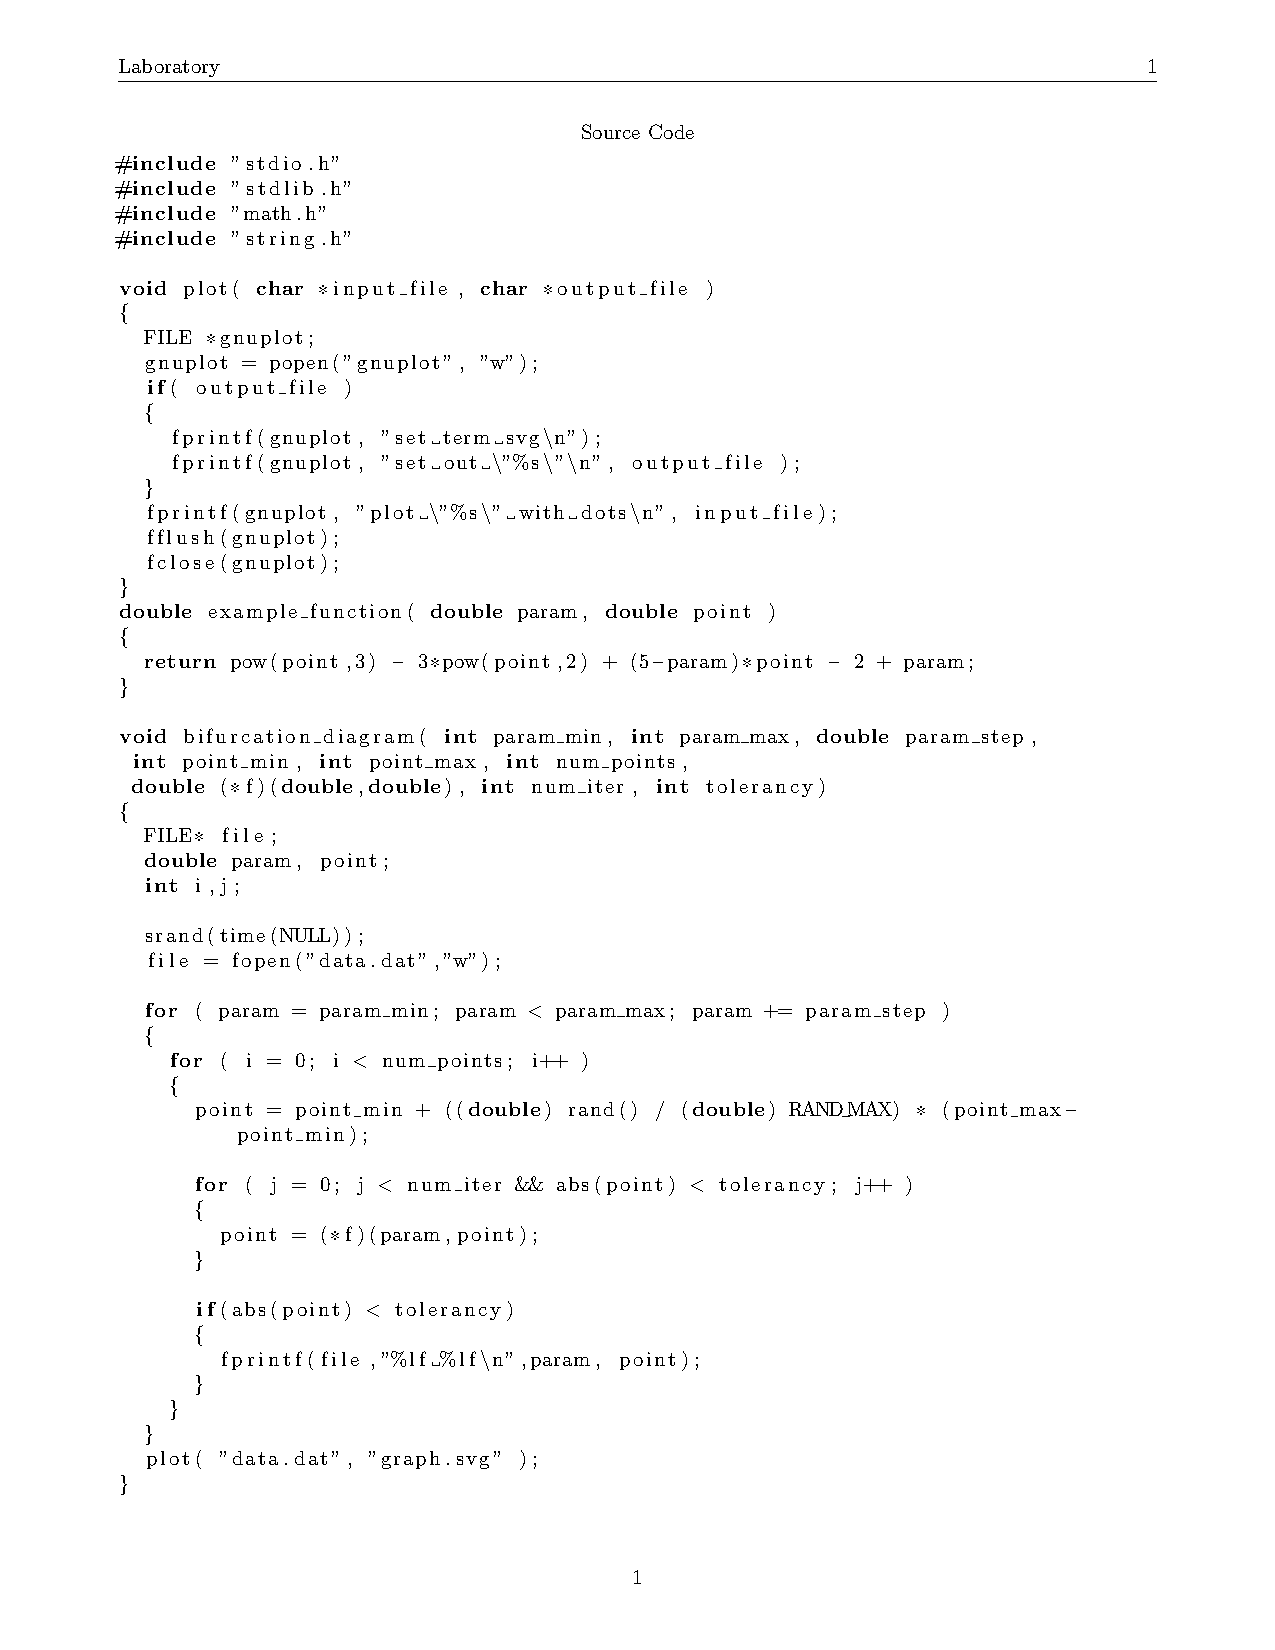
\includepdf[pages=-]{../Tasks/scripts/script3}

\end{document}